% % % % % % % % % % % % % % %
\documentclass[11pt]{article}
\usepackage[a4paper, portrait, margin=1in]{geometry}
% % % % % % % % % % % % % % %
\usepackage{graphicx}
\usepackage{listings}
\usepackage{epstopdf}
\usepackage{caption}
\usepackage{svg}
\usepackage{amsmath}
\usepackage{lscape}
\usepackage{multirow}

\newsavebox\IBoxA \newsavebox\IBoxB \newsavebox\IBoxC \newlength\IHeight
\newcommand\TriFig[9]{% Image1 Caption1 Label1 Image2 ...
	\sbox\IBoxA{\includegraphics[width=0.32\textwidth]{#1}}
	\sbox\IBoxB{\includegraphics[width=0.32\textwidth]{#4}}
	\sbox\IBoxC{\includegraphics[width=0.32\textwidth]{#7}}%
	\ifdim\ht\IBoxA>\ht\IBoxB
	\setlength\IHeight{\ht\IBoxB}\else\setlength\IHeight{\ht\IBoxA}\fi%
	\ifdim\ht\IBoxA>\ht\IBoxC
	\setlength\IHeight{\ht\IBoxC}\else\setlength\IHeight{\ht\IBoxA}\fi%
	\ifdim\ht\IBoxB>\ht\IBoxC
	\setlength\IHeight{\ht\IBoxC}\else\setlength\IHeight{\ht\IBoxB}\fi%  
	\begin{figure}[!htb]
		\minipage[t]{0.32\textwidth}\centering
		\includegraphics[height=\IHeight]{#1}
		\caption{#2}\label{#3}
		\endminipage\hfill
		\minipage[t]{0.32\textwidth}\centering
		\includegraphics[height=\IHeight]{#4}
		\caption{#5}\label{#6}
		\endminipage\hfill
		\minipage[t]{0.32\textwidth}\centering
		\includegraphics[height=\IHeight]{#7}
		\caption{#8}\label{#9}
		\endminipage
	\end{figure}%
}

\newcommand\TwoFig[6]{% Image1 Caption1 Label1 Image2 ...
	\sbox\IBoxA{\includegraphics[width=0.5\textwidth]{#1}}
	\sbox\IBoxB{\includegraphics[width=0.5\textwidth]{#4}}%
	\ifdim\ht\IBoxA>\ht\IBoxB
	\setlength\IHeight{\ht\IBoxB}\else\setlength\IHeight{\ht\IBoxA}\fi%
	\begin{figure}[!htb]
		\minipage[t]{0.5\textwidth}\centering
		\includegraphics[height=\IHeight]{#1}
		\caption{#2}\label{#3}
		\endminipage \hfill
		\minipage[t]{0.5\textwidth}\centering
		\includegraphics[height=\IHeight]{#4}
		\caption{#5}\label{#6}
		\endminipage
	\end{figure}%
}


\begin{document}

\title{Advanced Systems Lab (Fall'15) -- Second
Milestone}

\author{Name: \emph{Sandro Huber}\\Legi number: \emph{10-924-777}}

\date{
\vspace{4cm}
\textbf{Grading} \\
\begin{tabular}{|c|c|}
\hline  \textbf{Section} & \textbf{Points} \\ 
\hline  1 &  \\ 
\hline  2 &  \\ 
\hline  3.1 &  \\ 
\hline  3.2 &  \\ 
\hline  4 &  \\ 
\hline  5 &  \\ 
\hline \hline Total & \\
\hline 
\end{tabular} 
}

\maketitle

\newpage

\section*{Notes on writing the report}

The report does not need to be extensive but it must be concise, complete, and correct. Conciseness is important  in  terms  of  content  and explanations,  focusing  on  what  has  been  done and  explanations  of the results. A long report is not necessarily a better report, especially if there are aspects of the design or  the  experiments  that  remain  unexplained.  Completeness  implies  that  the  report  should  give  a comprehensive idea of what has been done by mentioning all key aspects of the modeling and analysis effort. You are allowed to modify the system designed in Milestone 1 (changes must be explained in the report)  and  you  can  run  new  experiments. If  you  have  been  told  that something  must  be corrected  in your system as a result of the evaluation of Milestone 1, please do so and indicate the corrections in the report. Limited analysis because of flaws in the system or lack of experimental data from milestone 1 are not  valid  arguments  for  an incomplete  report.  If  bugs  or  lack  of  data  prevent  you  from  doing  a  correct analysis, the system must be debugged and new data collected. 

Remember  that  this is  a  report  about modeling  and  analyzing the  system you  have  designed  and  built, using  the experimental data you have collected. There is no unique way to do the report and you may choose  to  focus  on  different  aspects  of  the  system  as  long  as  you deliver a  complete analysis of  its behavior. Please do not contact us seeking confirmation and assurances about, e.g., whether the report is  sufficient,  your  interpretation  of  the  data,  validation  of  concrete  aspects  of  your model, or  whether you have done enough experiments. Making those decisions is your job and part of what the course will evaluate. 

The milestone is worth 300 points. 

The report should be organized in sections as explained in the next pages, and each section should address at least the questions mentioned for each point. You might be called for a meeting in person to clarify aspects of the report or the system and to make a short presentation of the work done. By submitting the report, you  confirm  that  you  have  done  the  work  on  your  own,  the  data used comes  from  experiments  your have  done,  you  have  written  the  report  on  your  own,  and  you have  not  copied  neither text  nor  data from other sources.

\section*{Formatting guidelines}
While you can use any text processor of your choice for writing the report, please conform to the following formatting rules:
\begin{itemize}
\item  We expect you to submit \textbf{a single PDF that has the same section structure as this template} (if you use this file, you should remove this page with notes, and the short description provided by us at the beginning of sections).
\item  The main text should be in \textbf{single-column format with 11pt font on A4 paper}. In case you don't start with one of the files provided by us, \textbf{for margins use 2.54 cm (1 inch) on all sides}.
\end{itemize}

\pagebreak


\section{System as One Unit}\label{sec:system-one-unit}

\textbf{TODO: CLARIFY OPERATIONS VS REQUESTS (I.E.) 1 OPERATION = 5 REQUESTS, WHICH ONES? PLUS TELL THAT SLEEPTIME IS NEGLIBABLE IN IRTL PLOTS/CALCULATIONS}

Length: 1-2 pages

Build an M/M/1 model of your entire system based on the stability trace that you had to run for the first milestone. Explain the characteristics and behavior of the model built, and compare it with the experimental data. Analyze the modeled and real-life behavior of the system (explain the similarities, the differences, and map them to aspects of the design or the experiments).

The following numbers have been measured in the stability experiment 2, which only was ran for 120 seconds, since it was clear that the system itself is stably performing. All numbers are measured in the middleware, since this is the end and start of a request in the black box, which surrounds the middlewares and the database. To account for warmup and cooldown phase the first and last 10 seconds were ignored, such we end up with a 100 seconds of valid data. There were 2 middlewares and 1 database with 40 concurrent connections. Strangly the numbers from the milestone 1 couldn't be reached again, there was a constant shift by $\approx\frac{3}{5}$ over the whole data. So the bahaviour didn't change. The reason for this could be a higher network usage of the system or more distance between the individual machines hired. Because of the prizing and limited time budget I was not able to redo this experiment a third time.
\begin{center}
	\captionof{table}*{Measured Data} 
	\begin{tabular}{c|c}
		\hline
		Throughput $X$ & 554.94 Req/sec \\
		Response Time $R$ & 216.5 ms/Req \\
		Queueing Time $I$ & 142.6 ms/Req \\ \hline		
	\end{tabular}
\end{center}

\begin{center}
	\captionof{table}*{Calculated Data}
	\begin{tabular}{c|c}
		\hline
		Arrival Rate $\lambda$ & $X$* \\
		Service Time $S$ & 71.91 ms/Req \\
		Service Rate $\mu$ & 13.91 Req/sec \\
		Traffic Intensity $\rho$ & 39.91 \\
		\hline		
	\end{tabular}
\end{center}
\footnotesize*This holds, because the system built is a closed one. This is known, because every client first sends a request into the system and waits until an answer in form of a request comes back. Only then the client proceeds with it's job based on the meaning of the answer. If an answer is lost during transmission or execution the system will automatically take care of this and closes the socket connection to this client, such that it knows an error occured and it has to reconnect if there are still messages not successfully sent yet. This guarantees that no messages are no false positives when logging the throughput.
\normalsize
\newline\newline
Based on the following law:
\begin{equation}
	\text{System is stable}\Leftrightarrow \text{Traffic Intensity} < 1,
\end{equation}
\TwoFig {figures/stability_2/tp.eps} {Throughput of the whole System} {fig:stab2tp}
		{figures/stability_2/rt.eps} {Response Time per Request} {fig:stab2rt}
the system should be heavily unstable. But multiple factors show evidence that this is not the case. First we can have a look at the plots displayed in figures \ref{fig:stab2tp} and \ref{fig:stab2rt}. It's clearly visible that the system is stable. Another factor worth considering in view of this problem is the standard deviation of the throughput and response time which are $20.122$ Req/sec and $7.85$ ms/Req respectively. These two values are identical to $3.626\%$ (throughput) and $3.625\%$ (response time) variation with respect to the corresponding overall mean value, which again indicate a very stable system.

So how to explain then that the traffic intensity $\rho$ $=39.91>1$? The answer lies in the choice of the model. Since the system that was built, internally has a lot of parallelism and works with threads that execute along eachother, the simple M/M/1 model is not able to explain this complex structure and thus fails. The value of the traffic intensity is not random at all though. It is still somewhat connected to the inner structure of the system. Precisely I am talking about the number of database connections, which are constantly 40 during the whole experiment (20 per middleware). In practice this means that on the database, 40 concurrent threads were available which serve concurrently all queries sent from the middlewares. This would perfectly explain the traffic intensity, since when inserting these 40 concurrent threads into the equation: $\rho$ $=\frac{\lambda}{40\mu}=\frac{554.94 \text{ sec/Req}}{40*13.91\text{ Req/sec}}=\frac{554.94 \text{ sec/Req}}{556.4 \text{ Req/sec}}=0.9973<1$. To be sure that all 40 threads on the database are really in use the whole time, we can see if there is queueing happening in the right part of the system. Each request has to go to the database somewhen. The connections are provided through a connection pool. If there are currently no connections available, the request has to wait. In figure \ref{fig:queue_length} we can see that the queue length per middleware is on average of length $38.9$, which makes visible that indeed the database is the bottleneck. These numbers do make sense, because we now can precisely say in which state all the requests are: 40 requests are processed on the database and $2*38.9=77.8$ are waiting for a database connection. Because there were exactly 120 clients online (each one having one open request in the system and the sleep time of $\approx0.003ms$ is negligable) we know that we are missing track of $120-40-77.8=2.2$ requests on average. But this makes sense, because there have to be some requests on the way from the database back to the clients and some new ones coming from the clients which did not yet reach the database connection queue.
\begin{figure}
\centering
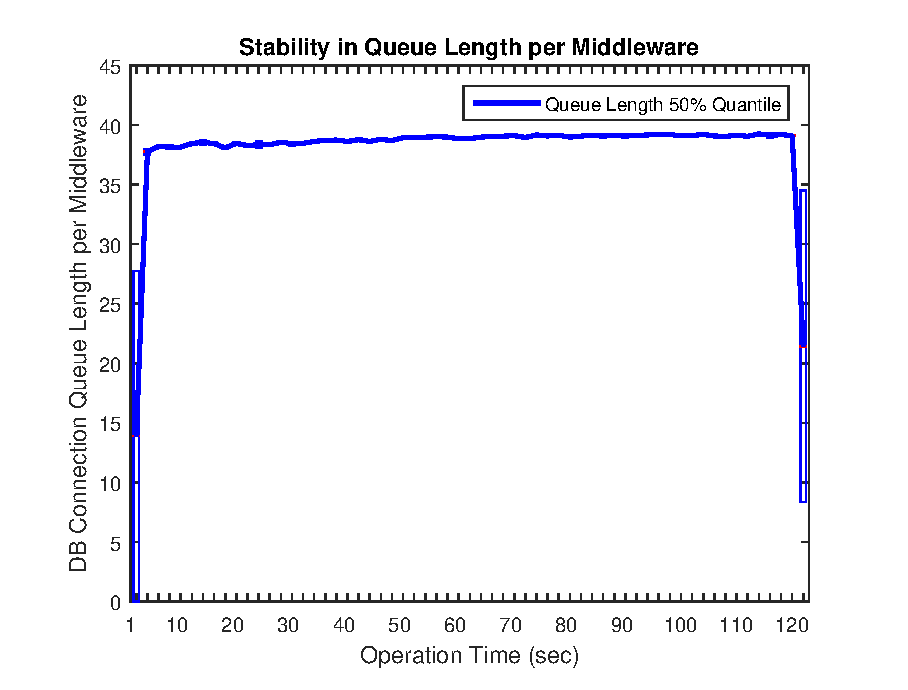
\includegraphics[width=0.5\linewidth]{figures/stability_2/queue_length}
\caption{Queue length in front of DB Connection pool}
\label{fig:queue_length}
\end{figure}

\section{Analysis of System Based on Scalability Data}\label{sec:analysis-scalability}

Length: 1-4 pages

Starting from the different configurations that you used in the first milestone, build queuing models of the system. Detail the characteristics of these series of models and compare them with experimental data. The goal is the analysis of the model and the real scalability of the system (explain the similarities, the 
differences, and map them to aspects of the design or the experiments).

The scalability of a system has two aspects: it describes the capability of the system to handle an increasing number of requests, but also the possibility of boosting the system performance by adding more modules. It's thus important to include both factors into the analysis. This is done by varying the number of clients as well as the number of middlewares. The number of clients ranged from 10 to 120 in steps of 10, whereas the number of middlewares were chosen to be either one or two. The reason for the client and middleware numbers are both based on benchmarks done in milestone 1. In short it holds that the database is the bottleneck and is saturated by already 60 clients in total operating on one middleware. To get the full picture, the range of possible values was enlarged. In case of two middlewares, the clients as well as the totally 40 database connections were evenly split among both. Let's analyse the first configuration with one middleware, all possible number of clients (evenly split among two client machines) and one database providing 40 concurrent connections.

Also based on benchmarks evaluated in milestone one, we can assume that the database is the bottleneck in this configuration. As in the book of Raj Jain is written, an M/M/m queue is used to model a multi-server system where jobs for these servers are kept in one queue. In our case, the servers are equal to the threads on the database and the single queue is found as the waiting queue for a database connection on the middleware. It thus make sense to apply an M/M/40 queueing model, because as said, the database provides 40 concurrent connections, and thus, internally runs 40 threads.

\begin{center}
	\captionof{table}*{M/M/40 Model on Scalability Data for 1 Middleware}
	\begin{tabular}{c|c|c||c|c|c}
		\hline
		& \multicolumn{2}{c||}{Model Parameters} & \multicolumn{3}{c}{Computed and Measured Variables} \\
		\hline
		\#Clients & $\lambda$ (Req/sec) & $\mu$ (Req/sec) & $\rho$ & $\varrho^{*_1}$(\%) & Queue Length$^{*_2}$ \\
		\hline
		10 & 2481.5 & 366.15 & 0.1694 & $2.5783*10^{-13}$ & 0.19\\
		20 & 4773.5 & 341.82 & 0.3491 & 1.15 & 0.40\\
		30 & 7015.5 & 339.42 & 0.5167 & 51.66 & 0.68\\
		40 & 9311.5 & 332.88 & 0.6993 & 69.93 & 0.90\\
		50 & 10346.5 & 303.02 & 0.8536 &85.36 & 1.36\\
		60 & 12302 & 317.06 & 0.9700 & 97.00 & 5.79\\
		70 & 13152 & 329.90 & 0.9967 & 99.67 & 21.31\\
		80 & 13005.5 & 326.25 & 0.9966 & 99.66  & 40.83\\
		90 & 12321 & 308.14 & 0.9996 & 99.96 & 61.68\\
		100 & 13383 & 335.71 & 0.9966 & 99.66 & 77.74\\
		110 & 13013.5 & 326.28 & 0.9971 & 99.71 & 99.13\\
		120 & 12642.5 & 316.59 & 0.9983 & 99.83 & 119.10\\
		\hline		
	\end{tabular}
	\captionof{table}*{$^{*_1}$: Probability of Queueing $^{*_2}$: Average per Request}
\end{center}

The first improvement of this model with respect to the simple M/M/1 model visible is the much better fit of the traffic intensity $\rho$. Indeed, the model does now also yield a stable system and thus is closer to reality. The model gives also reasonable insights into the probability of queueing happening. When we have values of the measured queue length which are $<1$, it means that more requests had an empty queue than requests which had another request actually waiting infront of them already.

\section{Modeling Components as Independent Units}\label{sec:independent-units}

Length: 1-5 pages

In this section you will build M/M/m models of the middleware and the database and explain the characteristics of both. As before, compare them with relevant experimental data and analyse the similarities and differences between models and real behaviour, and link these to specific design decisions in your system.

\subsection{Middleware}\label{sec:mw}
As already explained in the first Milestone, the middleware was built with maximal adaptivity to the current situation in mind. This means that a middleware is able to dynamically allocate resources on demand when either more clients join the system, or in general more requests are generated. To realize this feature, a \textit{cached thread pool} of the \textit{ExecutorService} class has been instantiated to deal with the distribution of requests to threads. The magic behind this class is that it automatically creates and runs threads for each new job, in our case requests, entering the middleware. As shown in the benchmarks for the middleware, this setup allows a very high throughput of around 45'000 requests per second. Since the behaviour of the \textit{cached thread pool} is not fully clear, because one just can't look into its source code, it's necessary to first understand the relationship between the two factors '\#Clients' and '\#Threads'. The number of requests is here not important, because it's not about the throughput (i.e. requests per second), but about the number of requests currently in the system, which is directly correlated to the number of clients.
\newline\underline{Configuration}: This analysis was done on the scalability data. There were one or two middlewares, one database with 40 concurrent connections and two client machines online which provided system access for clients. If two middlewares were online, the clients and database connections were evenly split among both. The clients sent as much as they could, following the load configuration mentioned in milestone 1. Each message had a content of length 200. The number of threads was measured by looping through all available threads and counting those which were in the state \textit{RUNNABLE}.
\newline\underline{Expectation}: The middleware structure is based on a two-step approach: Whenever a new requests enters the middleware, a new thread gets launched which handles the reading, deserialization and database access. When this is completed, this thread shuts down and fires up a second thread that handles the serialization of the answer and sends it back to the corresponding client. So in average there is one thread online per request. Thus we can expect that the equation $\text{'\#Requests in middleware or database'}=\text{'\#Request not in clients'}=\text{'\#Threads'}$ should hold. But in section \ref{sec:system-one-unit} we already saw that only a very small minority of requests is not found in the database or the middleware. With this reasoning we can expect the following behaviour for n clients: $\#Threads=n-\epsilon$, for $\epsilon>0$ and small.
\newline\underline{Reality} (figure \ref{fig:threads}): It's obvious that the mismatch between the measured number of threads and the expectation is serious. What went wrong? The whole analysis was based on the idea of having one thread per request in the middleware or database. But one thing I forgot was the ability of threads to get reused. For example when a request waits for a database connection, its corresponding thread can meanwhile be reused by another request for e.g. deserialization. It therefore holds that  $\text{'\#Requests in middleware or database'}=\text{'\#Request not in clients'}\neq\text{'\#Threads'}$. We still want to correlated the number of clients to the load of the middleware. Although the equation chain does not hold, we still can use its first part, namely $\text{'\#Requests in middleware or database'}=n-\epsilon=\text{'\#Clients'}-\epsilon$, for $\epsilon>0$ and small. By simply counting these requests which currently are processed by either the middleware or the database we end up with a much better fit onto the expectation (figure \ref{fig:refined_mw_load}). We indeed can see that the relation is linear and fulfills the expected bahaviour of $n\approx\text{'\#Requests in middleware or database'}$.

\TwoFig {figures/middleware/threads} {Number of Threads over all\\middlewares under different configurations}
		{fig:threads}
		{figures/middleware/req_vs_clients_on_mw} {Refined load estimation on the middleware} {fig:refined_mw_load}

The figure \ref{fig:refined_mw_load} does verify our assumption of having a linear load-dependent middleware behaviour. This is a problem for modelling, because fitting a single model won't be easy. So let's tackle this problem step by step. First, let's see if there is a model fitting onto every point of the middleware baseline, and in a second step, I try to unite these models into a single one. The first step is done, such that I get more insights into which models fit certain regions of the middleware behaviour and allow easier designing of the single M/M/m model. I quickly repeat the conditions of the middleware baseline:
\newline\underline{Configuration}: The middleware was as isolated as possible, i.e. no database access was made. Two client machines were flooding either one or two middlewares with messages with content length 200. As service time, only the time within the middleware was measured. To apply an M/M/m model, the throughput and service time of the corresponding experiment data were taken. To get an idea of how well different models fit onto the data I did the following: For every point i.e. throughput and response time for $n$ clients, all M/M/m models with m going from 1 to 110 were applied. Because the system was stable in all phases of the experiment, the traffic intensity allows to see how well a model does fit.
\newline\underline{Expectation}: As seen in figure \ref{fig:refined_mw_load}, the load seems to relate linearly to the number of clients, so I have no reason the expect anything else of the models.
\newline\underline{Reality} (figure \ref{fig:load_dependence}): It's clearly visible that the linear trend could be verified also when applying the models. Since the system was stable, but still trying to get as much throughput as possible, a traffic intensity of just below $1$ is expectable. The plot was generated with this assumption in mind. This leads to the basic formula of $|(\rho-1)|^{-1}$, which models the closeness to 1. To have a visually more appealing plot, the final formula reads as $\log(|(\rho-1)|^{-1}+4)$. Additionally to the linear relationship, it's noticeable, that models with higher m's tend to fit more parts of the whole data. This insight is used for the second step, when trying to fit a single model onto the data.

\TwoFig {figures/middleware/load_dependence} {Overview of how well the \\M/M/[1-110] models fit onto the\\ middleware data with respect to the traffic\\ intensity} {fig:load_dependence}
		{figures/middleware/mm95} {Applying the M/M/95 model onto the data of the middleware benchmark} {fig:mm95}

To test a single model onto the middleware, the response time yield by the model and the measured one will be compared. This will give a detailed insight into if and where the model does fit the built system. The approach taken is to model the middleware best when being under maximal load, i.e. when the throughput stagnates, but the response time still grows. This is the case when having 60 clients or more. By examining different models, the best one was found to be the M/M/95 model, which is displayed in figure \ref{fig:mm95}. The model is capable of not only representing the middleware when under maximal load, but also can closely predict the early stages when having a low load. The reason for not having the variance in the plot, is that I already worked with only the 50\% quantile of the data, because the throughput and response time data were logged in different settings (per requests and per second). But to generate a plot like the one seen in figure \ref{fig:mm95}, it's needed to have some sort of common structure. Coming back to the actual plot itself, why is it that exactly the M/M/95 model does the best job, and what is the relation to the real system? As mentioned in the in the first part of this section, threads are reused and thus can handle multiple requests. We saw in figure \ref{fig:threads} that the number of threads when having the maximal throughput, is on average 47 (calculated from the mean values of both settings 1 and 2 MW's). When calculating that the model does yield, that queueing happens with $83.88\%$ on average, we can assume that on average each thread can indeed handle multiple requests, because of the waiting induced by the queueing, but not too much, because of the only very limited time spent in the middleware ($<2.5ms$ on average). Eyeing at the M/M/95 model we can see that a re-usage factor of $\frac{95}{47}=2.02$ requests per thread would not only fit the model perfectly, but also does make sense with respect to the measured data.

\subsection{Database}\label{sec:db}
To find a queueing model for the database one has to take the hardware as well as the software setup into consideration. Let's first start with the hardware specification of the machine used during the experiments, since some of these led to later decisions in the experiment setup itself.

The database was run on a r3.4xlarge machine. By providing 122GiB of RAM it was guaranteed to have small tables fit into the working memory and get good performance. The machine also contained 8 physical CPU's which allows to have 16 parallel threads with hyper threading. By the rule of thumb presented by PostgreSQL itself it holds that the best optimal number of connections is $2*\text{'\#physical cores'}+C$, where $C$ is a constant. In the benchmark it was found that the best performance is reached with 20 concurrent database connections (position of the knee), i.e. the moment before the throughput stops to increase as rapid as in the beginning. Optimality in this context means to have the highest throughput with the least response time. It can be easily viewed in the corresponding figure in milestone 1, that optimal is not equal to maximal. In our case, the maximal throughput is reached when having around 40 database connections. This finding was the reason to run the experiments with 40 database connection if not mentioned otherwise. So from the software point of view we have 40 as an initial guess for the model parameter $m$. When searching through this model space ($m\in[20, 40]$), the best one to come across with respect to the mean squared error between the modelled and measured response time is M/M/30 with $0.0012$ ms of deviation. How is this model connected to the real system? Obviously 30 is exactly between our initial numbers gotten from the hard- and software evaluation, so intuitively it seems to fit. Basically it means, that although 40 threads are running, the performance does not much change with respect to the scenario when having only 30 clients, flooding the database with requests. Eyeing at the throughput plot in milestone 1, we can see that this is indeed the case. The reason for not quite reaching the same throughput as with 40 clients, is because the model does also try to fit onto the the system when it's not fully loaded and thus favours a smaller $m$. It also shows that in our case the rule of thumb does underestimate the power of the system. This can be explained, because the general rule of thumb assumes a default amount of work to be done for every request. In the load used in the experiments we have only one costly (pop message) and four cheap requests. This allows the system to perform better than expected and thus also exceed the lower bound of 20. The M/M/30 model allows to get more insights into how the database performs, for example when the machine starts to reach its performance boundaries.
\TwoFig {figures/database/mm30} {Applying the M/M/30 model onto\\ the data of the database benchmark} {fig:mm40}
		{figures/database/qprob} {Visualisation of the probability of queueing predicted by the M/M/30 model} {fig:qprob}
In figure \ref{fig:qprob} it's shown how the probability of queueing does behave when more clients are spamming requests to the database. The dashed red line indicates the 50\% border. Having data points above this line means, that on average queueing does happen more often than not. Queueing in the context of a database can be interpreted as waiting for a connection, when all connections are currently used. We can not only see that the queueing probability exceeds 50\% at around 30 clients and thus indicates that our choice of model is sound, but also that it's consistent with respect to the throughput measured in the first milestone, because it starts to decrease at around this many clients.
%\begin{figure}
%\centering
%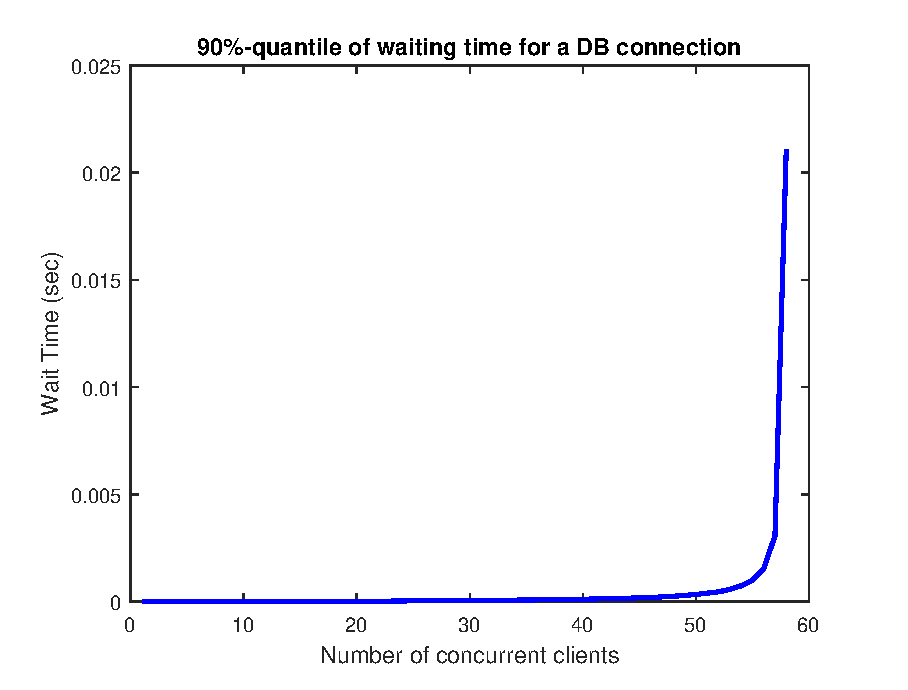
\includegraphics[width=0.7\linewidth]{figures/database/waittime}
%\caption{Estimated wait time for the M/M/30 model}
%\label{fig:waittime}
%\end{figure}

\section{System as Network of Queues}\label{sec:network-of-queues}

Length: 1-4 pages

Based on the outcome of the different modeling efforts from the previous sections, build a comprehensive network of queues model for the whole system. Compare it with experimental data and use the methods discussed in the lecture and the book to provide an in-depth analysis of the behavior. This includes the identification and analysis of bottlenecks in your system.

In the last three section, all important individual system parts have been modelled individually. We can now use this information to try to fit a model when combining the individual parts into a single system. To do this, a network of queues is built. To model my system i did choose to take one M/M/30 queue for modelling the database and a M/M/95 queue to simulate the behaviour of the middleware. The clients and the all network delays are packed into a single queue, because neither service time does change with different loads or is dependent on it's position in the system (e.g. before or after the middleware). All of these decision directly follow the results obtained in sections \ref{sec:mw} and \ref{sec:db}. The full setup is shown in figure \ref{fig:networkofqueues}.
\begin{figure}[!htb]
\centering
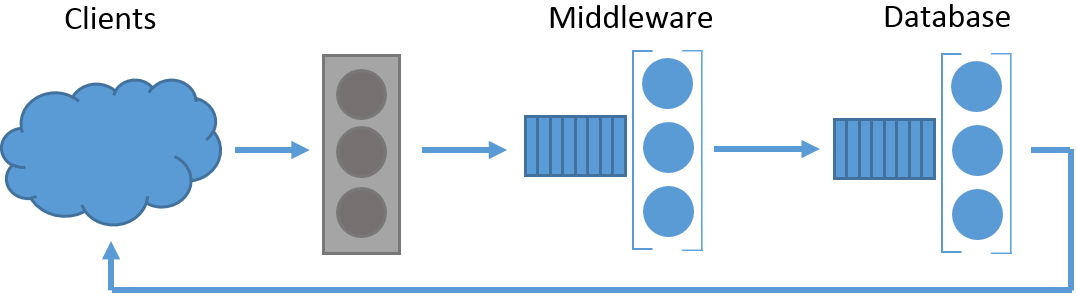
\includegraphics[width=1.0\linewidth]{figures/mva/networkofqueues}
\caption{Schematic setup of the Network of queues to simulate the behaviour of the whole system. The grey box corresponds to the delay center and the other ones to it's corresponding devices.}
\label{fig:networkofqueues}
\end{figure}
To proceed with the modelling, we need to find suitable input parameters for each of the devices. Since each component is modelled as own queue, these number can get extracted out of the baselines computed in the first milestone. The findings are summarized in the following table:

\begin{center}
	\captionof{table}{Fixed Model Parameters for 30 Clients} 
	\begin{tabular}{c|c}
		\hline
		Middleware Service Time & 0.844386 ms/req\\
		Database Service Time & 1.327447 ms/req \\
		Network delays & 0.864723 ms/req \\
		Sleep Time $Z$ & 0.0020 ms/req \\
		Parallelisation factor for Middleware & 95 \\
		Parallelisation factor for Middleware & 30 \\
		\hline
	\end{tabular}
\end{center}
The measurements shown in table 1 lead to the following device configuration which serve as input for the mean value analysis.
\begin{center}
	\captionof{table}{MVA Devices}
	\begin{tabular}{c|c|c|c|c}
		\hline
		System part & Service Time (ms/req) & Type & Parallelisation & \#Visits/req\\
		\hline
		Client + Network & 0.864723 & DC$^{*_1}$ & 1 & 1\\
		Middleware & 0.844386 & LDSC$^{*_2}$ & 95 & 1 \\
		Database & 1.327447 & LDSC & 30 & 1 \\
		\hline
	\end{tabular}
	\captionof{table}*{$^{*_1}$: Delay center $^{*_2}$: Load-dependent service center}
\end{center}

\begin{center}
	\captionof{table}*{MVA on Scalability Data for 1 Middleware}
	\begin{tabular}{c|c|c|c|c||c|c}
		\hline
		& \multicolumn{4}{c||}{Computed Values} & \multicolumn{2}{c}{Measured Values} \\
		\hline
		\#Clients & U$_{MW}$ & U$_{DB}$ & X (Req/sec) & R (ms) & X (Req/sec) & R (ms) \\
		\hline
		10 & 0.03 & 0.2 & 2505 & 3.98 & 2482 & 2.76 \\
		20 & 0.06 & 0.36 & 4496 & 4.44 & 4474 & 2.96 \\
		30 & 0.10 & 0.563 & 7004 & 4.28 & 7016 & 2.98 \\
		40 & 0.12 & 0.759 & 9322 & 4.29 & 9312 & 3.04 \\
		50 & 0.14 & 0.86 & 10453 & 4.78 & 10347 & 3.5 \\
		60 & 0.14 & 0.97 & 11180 & 5.36 & 12302 & 3.56 \\
		70 & 0.14 & 0.99 & 11124 & 6.29 & 13152& 4.02 \\
		80 & 0.14 & 0.97 & 11034 & 7.24 & 13006 & 4.81 \\
		90 & 0.14 & 0.99 & 11043 & 8.14 & 12321 & 5.94 \\
		100 & 0.14 & 0.99 & 11010 & 9.1 & 13383 & 6.06 \\
		110 & 0.14 & 0.99 & 10980 & 10.00 & 13014 & 7.06 \\
		120 & 0.14 & 0.99 & 10952 & 10.95 & 12643 & 8.05 \\
		\hline		
	\end{tabular}
\end{center}

\section{Interactive Law Verification}\label{sec:interactive-law}

Length: 1-2 pages

Check the validity of all experiments from milestone 1 using the interactive law. Analyze the results and explain them in detail.

mw baseline: with 1 cm interactive law does not fit the line, because with that setup the system was not closed? the client was not able to bring enough reqeuests, and started to block itself. thats way less throughput was registered and higher response times are expected, but not measured, because the middleware was not at it's limits yet.

stability: discrepancy at the beginning due to the high think time used to setup clients.

2k verification:

\begin{tabular}{c|c|c||c|c}
	TP(Req/s) & RT(ms) & IRL(ms) & Abs. Difference(ms) & Percentual Difference(\%) \\
	\hline
	12427 & 5.12 & 4.83 & 0.29 & 5.66 \\
	14707 & 3.87 & 4.08 & 0.21 & 5.43 \\
	11859 & 4.84 & 5.06 & 0.22 & 4.55 \\
	16133 & 3.66 & 3.72 & 0.06 & 1.64 \\
	12413 & 9.98 & 9.67 & 0.31 & 3.11 \\
	18233 & 7.07 & 6.58 & 0.49 & 6.93 \\
	13238 & 9.14 & 9.06 & 0.08 & 0.88 \\
	16428 & 6.97 & 7.30 & 0.33 & 4.73 \\
	13488 & 4.69 & 4.45 & 0.24 & 5.12 \\
	15954 & 3.87 & 3.76 & 0.11 & 2.84 \\
	12289 & 4.94 & 4.88 & 0.06 & 1.21 \\
	15855 & 4.19 & 3.78 & 0.41 & 9.76 \\
	13017 & 9.16 & 9.22 & 0.06 & 0.66 \\
	17701 & 6.57 & 6.78 & 0.21 & 3.20 \\
	13054 & 9.31 & 9.19 & 0.12 & 1.29 \\
	17619 & 6.73 & 6.81 & 0.08 & 1.19 \\
	\hline  
	&&& avg: 0.21 & avg: 3.64 \\
	\hline  
\end{tabular}

\TwoFig {figures/interactive_law/db_baseline} {IL on DB Baseline} {}
		{figures/interactive_law/db_data_baseline} {IL on DB Data Baseline} {}

\TwoFig {figures/interactive_law/db_data_baseline_third_index} {IL on DB Data Baseline with 3rd Index} {}
		{figures/interactive_law/mw_baseline} {IL on MW Baseline} {}
		
\TwoFig {figures/interactive_law/client_baseline} {IL on Client Baseline} {}
		{figures/interactive_law/stability} {IL on Stability} {}
		
\TwoFig {figures/interactive_law/rt_1cm} {IL on Client Baseline} {}
		{figures/interactive_law/rt_2cm} {IL on Stability} {}

\section*{Appendix: Repeated Experiments}

Length: up to 5 pages but \textbf{only needed if you repeated experiments}.

This is the place to show any repeated or additional experiments that you ran since milestone 1, for the reasons outlined in the description. If your previous submission had all necessary experiments for this milestone, remove the Appendix.

\TwoFig {figures/max_tp_2/tp} {} {}
		{figures/max_tp_2/rt} {} {}
	
\TwoFig {figures/db_1M_2/tp} {} {}
		{figures/db_1M_2/rt} {} {}

\TwoFig {figures/scalability/tp} {scalability} {}
		{figures/scalability/rt} {scalability} {}

\end{document}
